\chapter{Descrizione del Dataset}

\label{Capitolo 3}

\section{Provenienza del Dataset}

Il dataset utilizzato per il funzionamento dell'applicazione è stato costruito manualmente per intero. Una grande quantità di dati è stata estratta dalle seguenti fonti:
\begin{itemize}
    \item F1 2023, videogioco prodotto da CodeMaster e EA con licenza ufficiale della F1;
    \item F1 Manager 2023, videogioco manageriale sviluppato da Frontier Developments con licenza ufficiale della F1;
    \item \url{https://tracks.f1setup.it/}, che contiene informazioni dei vari circuiti;
    \item \url{https://www.statsf1.com/it}, che contiene un database su ogni attività in pista avvenuta dal 1951 in Formula1;
    \item \url{https://steamcommunity.com/sharedfiles/filedetails/?id=3033340960}, una guida che contiene le informazioni tecniche dei circuiti.
\end{itemize}
L’intero database è disponibile in formato .txt da eseguire tramite un compilatore SQL. È reperibile nella cartella \texttt{LMFP/tree/master/src/main/java/it/polito/tdp/SimulazioneF1/db}.

\section{Contenuto del Dataset}

Il dataset contiene principalmente dati e informazioni su:
\begin{itemize}
    \item valutazioni qualitative dei piloti attualmente ingaggiati dai team;
    \item valutazioni qualitative delle vetture di ogni scuderia;
    \item informazioni identificative dei piloti, sui team e sui circuiti;
    \item dati tecnici per ogni circuito presente nel calendario 2024 del campionato di F1;
    \item numero di sorpassi effettuati per ogni circuito nelle edizioni disputate dal 2010 al 2023 (compresi).
\end{itemize}

\section{Struttura e Descrizione delle Tabelle}

\begin{figure}[htbp]
    \centering
    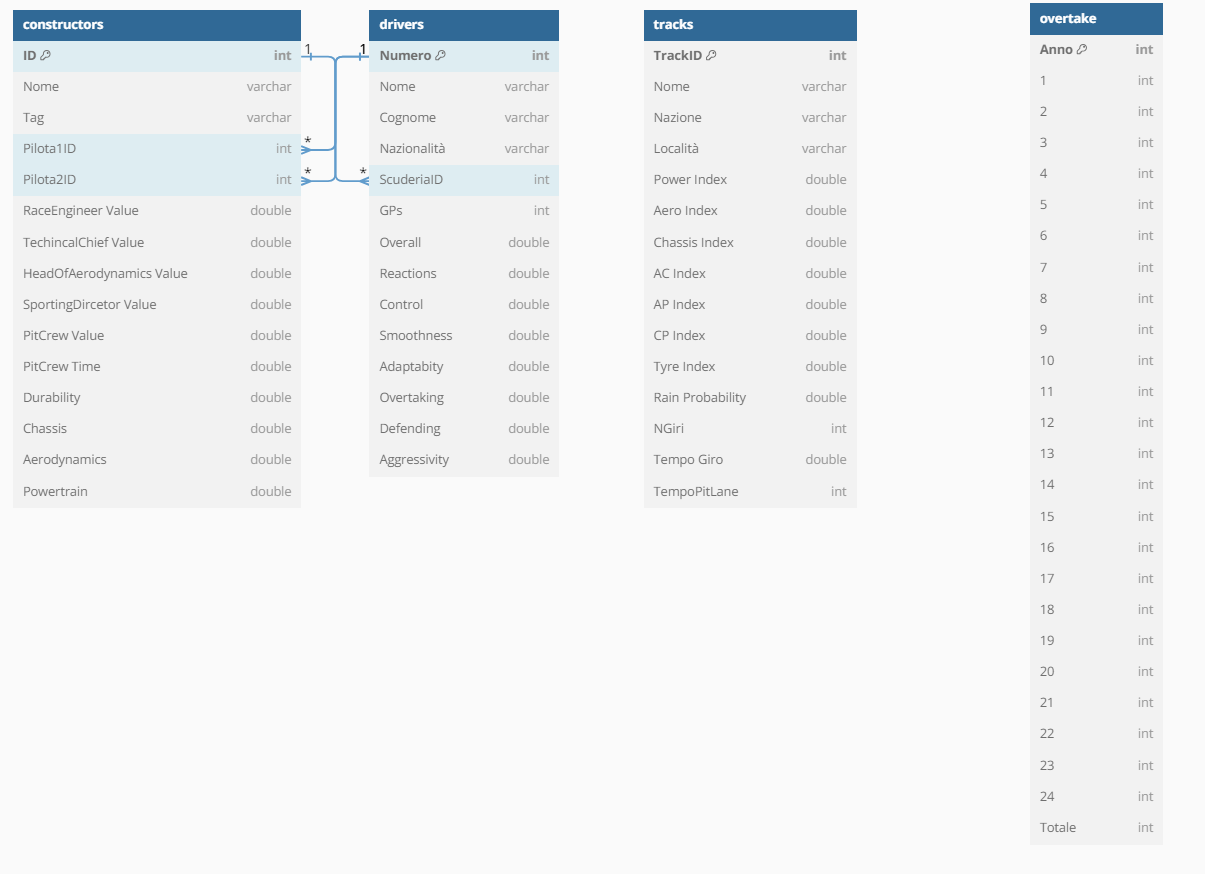
\includegraphics[width=\textwidth]{Figures/db.png}
    \caption{Diagramma di schema del database}
    \label{fig:database-schema}
\end{figure}

\subsection{Tabella Constructors}

La tabella \texttt{Constructors} contiene dati identificativi riguardanti i 10 team presenti attualmente in Formula 1 e dati qualitativi sulle rispettive vetture. \\
Descrizione delle colonne:
\begin{itemize}
    \item \texttt{ID}: numero che identifica univocamente il team;
    \item \texttt{Pilota1ID}: numero che descrive univocamente il pilota1 del team;
    \item \texttt{Pilota2ID}: numero che descrive univocamente il pilota2 del team;
    \item \texttt{Nome}: nome del team;
    \item \texttt{Tag}: abbreviazione di tre lettere del nome del team;
    \item \texttt{RaceEngineerValue}: indice qualitativo dell’ingegnere di gara del team;
    \item \texttt{TechnicalChiefValue}: indice qualitativo del capo dello sviluppo tecnico del team;
    \item \texttt{HeadOfAerodynamicsValue}: indice qualitativo del capo del settore aerodinamico del team;
    \item \texttt{PitCrewValue}: indice qualitativo sulla Pit Crew del team;
    \item \texttt{PitCrewTime}: tempo medio di pit stop effettuato dalla Pit Crew;
    \item \texttt{Durability}: indice qualitativo della resistenza dei componenti che costituiscono la vettura del team;
    \item \texttt{Chassis}: indice qualitativo del telaio della vettura del team;
    \item \texttt{Powertrain}: indice qualitativo del motore della vettura del team;
    \item \texttt{Aerodynamics}: indice qualitativo dell’aerodinamica della vettura del team;
\end{itemize}

\subsection{Tabella Drivers}

La tabella \texttt{Drivers} contiene dati identificativi sui 20 piloti che gareggiano attualmente in F1 e delle statistiche qualitative riguardo alle rispettive abilità di guida. \\
Descrizione delle colonne:
\begin{itemize}
    \item \texttt{Numero}: numero univoco che identifica la vettura che guida il pilota;
    \item \texttt{Nome}: nome del pilota;
    \item \texttt{Cognome}: cognome del pilota;
    \item \texttt{Nazionalità}: nazionalità del pilota;
    \item \texttt{ScuderiaID}: codice identificativo della scuderia del pilota;
    \item \texttt{GPs}: numero di GP disputati dal pilota prima dell’inizio della stagione 2024;
    \item \texttt{Overall}: indice qualitativo totale dell’abilità di guida del pilota;
    \item \texttt{Reactions}: indice sulla capacità di reazione ad imprevisti del pilota;
    \item \texttt{Control}: indice sul controllo in situazioni particolari della guida del pilota;
    \item \texttt{Smoothness}: indice sull’abilità di gestire le gomme del pilota;
    \item \texttt{Adaptability}: indice sull’abilità di adattamento del pilota;
    \item \texttt{Overtaking}: indice sull’abilità del sorpasso del pilota;
    \item \texttt{Defending}: indice sulla capacità di difesa del pilota;
    \item \texttt{Aggressivity}: indice sull’aggressività di guida del pilota;
\end{itemize}

\subsection{Tabella Tracks}

La tabella \texttt{Tracks} contiene dati identificativi del circuito, oltre agli indici che indicano quanto il circuito si presti ad una determinata qualità tecnica delle vetture (aerodinamica, telaio, motore). \\
Descrizione delle colonne:
\begin{itemize}
    \item \texttt{TrackID}: numero identificativo univoco del circuito;
    \item \texttt{Nome}: nome esteso del circuito;
    \item \texttt{Nazione}: nazione in cui è situato il circuito;
    \item \texttt{Località}: località in cui è situato il circuito;
    \item \texttt{Power Index}: indice sull’importanza del motore sulla prestazione nel circuito;
    \item \texttt{Aero Index}: indice sull’importanza dell’aerodinamica sulla prestazione nel circuito;
    \item \texttt{Chassis Index}: indice sull’importanza del telaio sulla prestazione nel circuito;
    \item \texttt{AC Index}: indice di correlazione sull’importanza aerodinamica - telaio sulla prestazione nel circuito;
    \item \texttt{AP Index}: indice di correlazione sull’importanza aerodinamica - motore sulla prestazione nel circuito;
    \item \texttt{CP Index}: indice di correlazione sull’importanza motore - telaio sulla prestazione nel circuito;
    \item \texttt{Tyre Index}: indice sul consumo gomma del circuito;
    \item \texttt{Rain Probability}: probabilità di pioggia sul circuito;
    \item \texttt{NGiri}: numero di giri della gara disputata sul circuito;
    \item \texttt{Tempo Giro}: tempo in secondi di percorrenza in condizioni ideali del circuito;
    \item \texttt{TempoPitLane}: tempo medio in secondi di percorrenza della Pit Lane del circuito durante un pit stop;
\end{itemize}

\subsection{Tabella Overtake}

La tabella \texttt{Overtake} contiene il numero di sorpassi effettuati in un circuito per ogni anno nelle gare disputate dal 2010 al 2023 (compresi). La tabella è stata creata con i codici identificativi dei circuiti come colonne per facilitare l’estrazione e l’analisi dei dati. È utilizzata solamente per calcolare un indice di probabilità di sorpasso, attributo di un’istanza Circuito.


